\documentclass[12pt]{article}
\usepackage[left=1cm, right=1cm, top=2cm,bottom=1.5cm]{geometry} 

\usepackage[parfill]{parskip}
\usepackage[utf8]{inputenc}
\usepackage[T2A]{fontenc}
\usepackage[russian]{babel}
\usepackage{enumitem}
\usepackage[normalem]{ulem}
\usepackage{amsfonts, amsmath, amsthm, amssymb, mathtools}
\usepackage{tikz}
\usepackage{tabularx}
\usepackage{hhline}

\usepackage{accents}
\usepackage{fancyhdr}
\pagestyle{fancy}
\renewcommand{\headrulewidth}{1.5pt}
\renewcommand{\footrulewidth}{1pt}

\usepackage{graphicx}
\usepackage[figurename=Рис.]{caption}
\usepackage{subcaption}
\usepackage{float}

%%Наименование папки откуда забирать изображения
\graphicspath{ {./images/} }

%%Изменение формата для ввода доказательства
\renewcommand{\proofname}{$\square$  \nopunct}
\renewcommand\qedsymbol{$\blacksquare$}

%%Изменение отступа на таблицах
\addto\captionsrussian{%
	\renewcommand{\proofname}{$\square$ \nopunct}%
}
%% Римские цифры
\newcommand{\RN}[1]{%
	\textup{\uppercase\expandafter{\romannumeral#1}}%
}

%% Для удобства записи
\newcommand{\MR}{\mathbb{R}}
\newcommand{\MQ}{\mathbb{Q}}
\newcommand{\MC}{\mathbb{C}}
\newcommand{\MK}{\mathbb{K}}
\newcommand{\MI}{\mathrm{I}}
\newcommand{\MJ}{\mathrm{J}}
\newcommand{\MH}{\mathrm{H}}
\newcommand{\MT}{\mathrm{T}}
\newcommand{\MU}{\mathcal{U}}
\newcommand{\MV}{\mathcal{V}}
\newcommand{\VN}{\varnothing}
\newcommand{\VE}{\varepsilon}
\newcommand{\id}{\mathrm{id}}
\newcommand{\Mat}{\text{Mat}}
\newcommand{\RE}{\operatorname{Re}}
\newcommand{\IM}{\operatorname{Im}}

\theoremstyle{definition}
\newtheorem{defn}{Опр:}
\newtheorem{rem}{Rm:}
\newtheorem{prop}{Утв.}
\newtheorem{exrc}{Упр.}
\newtheorem{lemma}{Лемма}
\newtheorem{theorem}{Теорема}
\newtheorem{corollary}{Следствие}

\newenvironment{cusdefn}[1]
{\renewcommand\thedefn{#1}\defn}
{\enddefn}

\DeclareRobustCommand{\divby}{%
	\mathrel{\text{\vbox{\baselineskip.65ex\lineskiplimit0pt\hbox{.}\hbox{.}\hbox{.}}}}%
}
%Короткий минус
\DeclareMathSymbol{\SMN}{\mathbin}{AMSa}{"39}
%Длинная шапка
\newcommand{\overbar}[1]{\mkern 1.5mu\overline{\mkern-1.5mu#1\mkern-1.5mu}\mkern 1.5mu}
%Функция знака
\DeclareMathOperator{\sgn}{sgn}

%Операторы ядра и образа
\DeclareMathOperator{\Ker}{Ker}
\DeclareMathOperator{\Ima}{Im}
\DeclareMathOperator{\tr}{tr}


%% Шапка для букв сверху
\newcommand{\wte}[1]{\widetilde{#1}}

%Обозначение константы
\DeclareMathOperator{\const}{\text{const}}

%Интеграл в большом формате
\DeclareMathOperator{\dint}{\displaystyle\int}
\newcommand{\ddint}[2]{\displaystyle\int\limits_{#1}^{#2}}


\newcommand{\smallerrel}[1]{\mathrel{\mathpalette\smallerrelaux{#1}}}
\newcommand{\smallerrelaux}[2]{\raisebox{.1ex}{\scalebox{.75}{$#1#2$}}}

\newcommand{\smallin}{\smallerrel{\in}}
\newcommand{\smallnotin}{\smallerrel{\notin}}

\newcommand*{\medcap}{\mathbin{\scalebox{1.25}{\ensuremath{\cap}}}}%
\newcommand*{\medcup}{\mathbin{\scalebox{1.25}{\ensuremath{\cup}}}}%

%Скалярное произведение
\DeclarePairedDelimiterX{\inner}[2]{\langle}{\rangle}{#1, #2}

%Подпись символов снизу
\newcommand{\ubar}[1]{\underaccent{\bar}{#1}}

\newcommand*\circled[1]{\tikz[baseline=(char.base)]{
		\node[shape=circle,draw,inner sep=2pt] (char) {#1};}}


\begin{document}
\lhead{Линейная алгебра}
\chead{Мануйлов В.М.}
\rhead{Лекция - 6}

\section*{Неравенство Коши-Буняковского}
\begin{defn}
	\uwave{Длиной} $a \in V$ будем называть $\sqrt{(a,a)} \geq 0$, обозначение $|a|$.
\end{defn}
\begin{theorem}(\textbf{Неравенство Коши-Буняковского})
	Пусть $V$ - линейное пространство над $\MK$, тогда будет верно следующее неравенство:
	$$
		\forall a,b \in V, \, |(a,b)| \leq |a|{\cdot}|b|
	$$ 
	где $|(a,b)|$ - модуль скаларного произведения, а $|a|, |b|$ - длины векторов $a$ и $b$.
\end{theorem}
\begin{proof}
	Докажем теорему для двух случаев $(1)$ $\MK = \MR$ и $(2)$ $\MK = \MC$. Пусть $a,b \in V$ - произвольные.
	
	$(1)$ $\forall t \in \MR$ возьмем $a + tb \Rightarrow (a + tb, a + tb) = (a,a) + 2t(a,b) + t^2(b,b) \geq 0$. Возможно два случая:
	\begin{enumerate}[label=\alph*)]
		\item $b = 0 \Rightarrow (a,b) = 0, \, |b| = 0 \Rightarrow |0| = 0 \leq |a|{\cdot}0 = 0 \Rightarrow$ неравенство выполняется;
		\item $b \neq 0 \Rightarrow (b,b) > 0, \, D = 4(a,b)^2 - 4(a,a){\cdot}(b,b) \leq 0 \Leftrightarrow (a + tb, a + tb) \geq 0$. Таким образом:
		$$
			(a,b)^2 \leq (a,a){\cdot}(b,b) \Leftrightarrow |(a,b)| \leq \sqrt{(a,a)}{\cdot}\sqrt{(b,b)} = |a|{\cdot}|b|
		$$
		требуемое неравенство выполняется;
	\end{enumerate}

	$(2)$ $\forall t \in \MC$ возьмем $a + tb \Rightarrow (a + tb, a + tb) = (a,a) + (a,tb) + (tb,a) + |t|^2{\cdot}(b,b)$, поскольку верно следующее:
	$$
		(\lambda a,b) = \overline{(b,\lambda a)} = \overline{\lambda}{\cdot}\overline{(b,a)} = \overline{\lambda}{\cdot}(a,b), \, t{\cdot}\overline{t} = |t|^2, \, (tb,tb) = t{\cdot}\overline{t}(b,b) = |t|^2{\cdot}(b,b) \Rightarrow
	$$
	$$
		\Rightarrow (a + tb, a + tb) = (a,a) + t{\cdot}(a,b) + \overline{t}{\cdot}\overline{(a,b)} + |t|^2{\cdot}(b,b)
	$$
	Подберем $t \colon t{\cdot}(a,b) \in \MR$. Вспомним, что $z = |z|e^{i\varphi} \Rightarrow (a,b) = |(a,b)|e^{i\varphi} \Rightarrow t = se^{-i\varphi}$, где $s \in \MR$, тогда:
	$$
		t{\cdot}(a,b) = |(a,b)|se^{-i\varphi}e^{i\varphi} = s|(a,b)| \Rightarrow |t| = |s|{\cdot}|e^{-i\varphi}| = |s| \Rightarrow |t|^2 = |s|^2 = s^2
	$$
	$$
		\overline{t}{\cdot}\overline{(a,b)} =|\overline{(a,b)}|e^{-i\varphi}\overline{s}e^{i\varphi} = |(a,b)|s		\Rightarrow
	$$
	$$
		\Rightarrow (a + tb, a + tb) = (a,a) + 2s{\cdot}|(a,b)| + s^2{\cdot}(b,b) \in \MR
	$$
	Все элементы принадлежат $\MR \Rightarrow D \leq 0 \Leftrightarrow |(a,b)|^2 \leq (a,a){\cdot}(b,b) = |a|^2{\cdot}|b|^2$.
\end{proof}

\begin{corollary}
	$\forall a,b \in V$ в Евклидовом случае $-1 \leq \dfrac{(a,b)}{|a|{\cdot}|b|} \leq 1$.
\end{corollary}
\begin{defn}
	\uwave{Углом между} $a$ и $b$ называется $\varphi_{ab} = \arccos\left(\dfrac{(a,b)}{|a|{\cdot}|b|}\right)$, в частности, если $(a,b) = 0$, то $a\bot b$.
\end{defn}
\begin{corollary}(\textbf{Неравенство треугольника})
	Пусть $V$ - линейное пространство над полем $\MK = \MC$, тогда верно:
	$$
		\forall a,b \in V, \, |a + b| \leq |a| + |b|
	$$
\end{corollary}
\begin{proof}
	$$
		\forall a,b \in V, \, |a + b| \leq |a| + |b| \Leftrightarrow (a + b, a+ b) \leq (|a| + |b|)^2 = |a|^2 + |b|^2 + 2|a|{\cdot}|b| \Leftrightarrow
	$$
	$$
		\Leftrightarrow (b,a) + (a,b) \leq 2|a|{\cdot}|b| \Leftrightarrow \overline{(a,b)} + (a,b) \leq 2|a|{\cdot}|b| 
	$$
	поскольку $z \in \MC \Rightarrow z = (a,b) = \RE{(a,b)} + i{\cdot}\IM{(a,b)} \Rightarrow \overline{(a,b)} + (a,b) = 2 \RE{(a,b)}$
	и $\RE{z} \leq |z|$, тогда:
	$$
		\overline{(a,b)} + (a,b) \leq 2|a|{\cdot}|b| \Leftrightarrow 2 \RE{(a,b)} \leq 2|a|{\cdot}|b| \Leftrightarrow \RE{(a,b)} \leq |(a,b)| \leq |a|{\cdot}|b|
	$$
	где в последнем слагаемом мы применили неравенство Коши-Буняковского.
\end{proof}
\begin{lemma}
	Пусть $a_1, \dotsc, a_n \neq 0$ и ортогональны (взаимно перпендикулярны). Тогда $a_1,\dotsc, a_n$ - линейно независимы.
\end{lemma}
\begin{proof}
	$\lambda_1 a_1 + \dotsc + \lambda_n a_n = 0$, обе части умножим на $a_i$ (скалярно) $\Rightarrow (a_i,\lambda_1 a_1 + \dotsc + \lambda_n a_n ) = (a_i, 0) = 0$, распишем второй аргумент подробнее:
	$$
		\lambda_1(a_i,a_1) + \dotsc + \lambda_i (a_i, a_i) + \dotsc + \lambda_n(a_i, a_n) = \lambda_i{\cdot}|a_i|^2 = 0 
	$$
	Поскольку $\forall i = \overline{1,n}, \, a_i \neq 0 \Rightarrow |a_i|^2 \neq 0 \Rightarrow \lambda_i = 0 \Rightarrow a_1,\dotsc, a_n$ - линейно независимы.
\end{proof}
\begin{defn}
	Система векторов $a_1,\dotsc, a_n$ называется \uwave{ортогональной}, если все $a_i \neq 0$ и $a_i \bot a_j, \, \forall i \neq j$. 
\end{defn}
\begin{defn}
	Система векторов $a_1,\dotsc, a_n$ называется \uwave{ортонормированной}, если она ортогональна и длина каждого вектора равна единице: $|a_1| = \dotsc = |a_n| = 1$.
\end{defn}

\section*{Ортогонализация Грама-Шмидта}


\begin{theorem}(\textbf{Процесс ортогонализации})
	Пусть $e_1, \dotsc, e_n$ - линейно независимы, тогда существует ортогональная система векторов $a_1,\dotsc, a_n$ такая, что $\langle a_1, \dotsc, a_k \rangle = \langle e_1, \dotsc, e_k \rangle, \, \forall k$.
\end{theorem}
\begin{proof}
	Пусть $e_1,\dotsc, e_n$ линейно независимый набор векторов, образуют цепочку линейных подпространств:
	$$
		V_1 = \langle e_1\rangle, \, V_2 = \langle e_1, e_2\rangle, \dotsc , V_n = \langle e_1, \dotsc, e_n\rangle, \,  V_1 \subset V_2 \subset \dotsc \subset V_n, \, \dim{V_i} = i
	$$
	Осуществим процесс ортогонализации по шагам:
	
	$(1)$ Пусть $a_1 = e_1, \, a_2 = e_2 + \lambda e_1 \Rightarrow (a_1, a_2) = 0 \Leftrightarrow (e_1, e_2 + \lambda e_1) = 0 \Leftrightarrow (e_1, e_2) + \lambda(e_1,e_1) = 0$, тогда $\lambda$ можно найти только в случае, если $(e_1,e_1) \neq 0$. Поскольку $e_1, \dotsc, e_n$ - линейно независимы, то $e_1 \neq 0$, следовательно $(e_1, e_1) = |e_1|^2 \neq 0$. Получается, что $a_1 \bot a_2$, $\langle a_1, a_2\rangle = \langle e_1, e_2\rangle = V_2$.
	
	$(2)$ Пусть $a_1, \, a_2$ уже найдены, ищем $a_3$ в виде: $a_3 = e_3 + \alpha a_1 + \beta a_2$, тогда рассмотрим систему:
	$$
		\left\{\begin{array}{ccc}
			(a_1,a_3) & = & 0\\
			(a_2,a_3) & = & 0\\
		\end{array}\right. \Leftrightarrow 
		\left\{\begin{array}{ccccc}
			(a_1,e_3 + \alpha a_1 + \beta a_2) & = & (a_1, e_3) + \alpha(a_1,a_1) + \beta(a_1,a_2) & = & 0\\
			(a_2,e_3 + \alpha a_1 + \beta a_2) & = & (a_2, e_3) + \alpha(a_2,a_1) + \beta(a_2,a_2) & = & 0
		\end{array}\right.
	$$
	Поскольку $a_1 \bot a_2$, то $(a_1, a_2) = (a_2,a_1) = 0$ и $(a_1,a_1) \neq 0 ,\, (a_2,a_2) \neq 0 \Rightarrow$ получим систему вида:
	$$
		\left\{\begin{array}{ccc}
			(a_1, e_3) + \alpha(a_1,a_1)  & = & 0\\
			(a_2, e_3) + \beta(a_2,a_2) & = & 0
		\end{array}\right.
	$$
	Она имеет решение $\Rightarrow$ мы нашли $a_3$. $V_3 = \langle e_1, e_2, e_3\rangle$
	
	$(3)$ Пусть мы нашли таким образом $a_1, \dotsc, a_k$. Рассматриваем $a_{k+1} = e_{k+1} + \lambda_1 a_1 + \dotsc + \lambda_k a_k \Rightarrow$ получим систему:
	$$
		\left\{\begin{array}{ccccc}
			(a_1,a_{k+1}) & = & (a_1, e_{k+1}) + \lambda_1(a_1,a_1) + \dotsc + \lambda_k(a_1,a_k) & = & 0\\
			\vdots & \vdots & \vdots & \vdots & \vdots\\
			(a_k,a_{k+1}) & = & (a_k, e_{k+1}) + \lambda_1(a_k,a_1) + \dotsc + \lambda_k(a_k,a_k) & = & 0
		\end{array}\right.
	$$
	Поскольку $\forall i = \overline{1,k}, \, (a_k,a_k) \neq 0$ и $\forall i \neq j, \, i,j = \overline{1,k}, \, (a_i,a_j) = 0$, то получим следующую систему:
	$$
		\left\{\begin{array}{ccc}
			(a_1, e_{k+1}) + \lambda_1(a_1,a_1)  & = & 0\\
			\vdots & \vdots & \vdots\\
			(a_k, e_{k+1}) + \lambda_k(a_k,a_k) & = & 0
		\end{array}\right.	
	$$
	Решение этой системы существует, если $|a_1| \neq 0, \dotsc, |a_k| \neq 0$. Надо проверить, что ни на каком шаге мы не сможем получить $a_i = 0$. Пусть $a_1 = e_1 \neq 0$ и $a_i = e_i + \mu_1 a_1 + \dotsc + \mu_{i-1}a_{i-1} = 0$. Воспользуемся тем, что $\langle a_1, \dotsc, a_{i-1} \rangle = \langle e_1, \dotsc, e_{i-1} \rangle$, тогда:
	$$
		\mu_1 a_1 + \dotsc + \mu_{i-1}a_{i-1} = \nu_1 e_1 + \dotsc + \nu_{i-1}e_{i-1} \Rightarrow e_i + \nu_1 e_1 + \dotsc + \nu_{i-1}e_{i-1} = 0 
	$$
	Тогда $e_1, \dotsc, e_i$ - линейно зависимы $\Rightarrow$ получили противоречие с $e_1, \dotsc, e_n$ - линейно независимы.
\end{proof}

Как выглядит матрица перехода от $e_1,\dotsc, e_n$ к $a_1, \dotsc, a_n$?
$$
	a_{k+1} = e_{k+1} + \lambda_1 a_1 + \dotsc + \lambda_k a_k \Rightarrow C = \begin{pmatrix}
		1 & * & \dotsc & * & *\\
		0 & 1 & \dotsc & * & * \\
		\vdots & \vdots & \ddots & \vdots & \vdots\\
		0 & 0 & \dotsc & 0 & 1 
	\end{pmatrix}
$$
Таким образом, матрица перехода $C$ - верхнетреугольная. 

\begin{defn}
	Пусть $L \subset V$ - линейное подпространство. \uwave{Ортогональным дополнением} $L^\bot$ к $L$ назовем следующее множество: 
	$$
		\{a \in V \colon (a,b) = 0, \, \forall b \in L\}
	$$
\end{defn}
\begin{lemma}
	Ортогональное дополнение является линейным подпространством.
\end{lemma}
\begin{proof}
	Проверим свойства подпространства:
	\begin{enumerate}[label ={(\arabic*)}]
		\item $\forall a_1, a_2 \in L^\bot, \, \forall b \in L$, $(a_1 + a_2, b) = (a_1,b) + (a_2,b) = 0  \Rightarrow a_1 + a_2 \in L^\bot$;
		\item $\forall a \in L^\bot, \, \forall b \in L, \, \lambda \in \MK \Rightarrow (\lambda{\cdot}a,b) = \begin{cases}
			\lambda{\cdot}(a,b), \, \MK = \MR \\
			\overline{\lambda}{\cdot}(a,b), \, \MK = \MC
		\end{cases} = 
		\begin{cases}
			0, \, \MK = \MR\\
			0, \, \MK = \MR
		\end{cases} \Rightarrow \lambda{\cdot}a \in L^\bot
	$;
	\end{enumerate}
\end{proof}
\begin{lemma}
	$V = L \oplus L^\bot$;
\end{lemma}
\begin{proof}
	Выберем произвольный базис в $L \colon e_1, \dotsc, e_k$ и дополним его до базиса $V \colon e_1, \dotsc, e_k, e_{k+1} ,\dotsc, e_n$. Применим процесс ортогонализации Грама-Шмидта $\Rightarrow$ получим $a_1, \dotsc, a_k, a_{k+1}, \dotsc, a_n$ - ортогональный базис $V \Rightarrow \langle e_1, \dotsc, e_k \rangle = \langle a_1, \dotsc, a_k \rangle \Rightarrow a_1, \dotsc a_k$ - ортогональный базис $L$. 
	
	Покажем, что $a_{k+1}, \dotsc, a_n$ - базис $L^\bot$.
	\begin{enumerate}[label ={(\arabic*)}]
		\item $\forall i > k, \, a_i \in L^\bot$ поскольку $a_i \in L^\bot \Leftrightarrow \forall b \in L, \, (a_i,b) = 0$, проверим:
		$$
	 		b \in L \Rightarrow b = \lambda_1a_1 + \dotsc + \lambda_k a_k \Rightarrow (a_i,b) = (a_i, \lambda_1 a_1 + \dotsc + \lambda_k a_k) = \lambda_1 (a_i, a_1) + \dotsc + \lambda_k (a_i, a_k) = 0
		$$
		в силу того, что $\forall j = \overline{1,k}, \, \forall i > k, \, (a_i, a_j) = 0$. Таким образом $\forall a_i \colon i > k \Leftrightarrow a_i \in L^\bot$;
		\item \uwave{Линейная независимость}: очевидно по построению;
		\item \uwave{Максимальность}: Пусть $a \in L^\bot \subset V \Rightarrow$ разложим $a$ по базису $V$:
		$$
			a = \alpha_1 a_1 + \dotsc + \alpha_k a_k + \alpha_{k+1}a_{k+1} + \dotsc + \alpha_n a_n
		$$
		Учитывая, что $a \in L^\bot \Leftrightarrow \forall b \in L, \, (a,b) = 0$, подставим $a_i, \, i \leq k$ вместо $b$, тогда получим:
		$$
			(a,a_i) = \overline{\alpha}_1(a_1, a_i) + \dotsc + \overline{\alpha}_k(a_k,a_i) + \overline{\alpha}_{k+1}(a_{k+1},a_i) + \dotsc + \overline{\alpha}_n(a_n,a_i) = 0 \Rightarrow \forall i \leq k, \, \alpha_i =0 \Rightarrow
		$$
		$$
			\Rightarrow \forall a \in L^\bot, \, a = \alpha_{k+1} a_{k+1} +  \dotsc + \alpha_n a_n
		$$
		Следовательно, получили максимальность;
	\end{enumerate}
	Таким образом, $a_{k+1}, \dotsc, a_n$ - базис в $L^\bot$. Покажем, что $V = L + L^\bot$:
	$$
		 \forall v \in V \Rightarrow v = v_1a_1 + \dotsc + v_k a_k + v_{k+1} a_{k+1} + \dotsc + v_n a_n
	$$
	$$
		v_1^L = v_1a_1 + \dotsc + v_k a_k \in L, \, v_2^{L^\bot} =  v_{k+1} a_{k+1} + \dotsc + v_n a_n \in L^\bot, \, v = v_1^L + v_2^{L^\bot}
	$$
	Покажем, что $V = L \oplus L^\bot$. Сумма прямая, если $L \cap L^\bot = \{0\}$, пусть $a \in L \cap L^\bot$, тогда:
	$$
		\forall b \in L, \, (a,b) = 0 \Leftrightarrow a \in L^\bot \Rightarrow b = a \in L \Rightarrow (a,a) = 0 \Leftrightarrow a = 0
	$$
\end{proof}
\begin{lemma}
	Пусть $V = L_1 \oplus L_2$, тогда $\forall a \in V, \, \exists !$ разложение $a = a_1 + a_2$, где $a_1 \in L_1, \, a_2 \in L_2$.
\end{lemma}
\begin{proof}(От противного):
	Пусть $a = a_1 + a_2 = b_1 + b_2, \, a_1,b_1 \in L_1, \, a_2,b_2 \in L_2 \Rightarrow (a_1 - b_1) = (a_2 - b_2)$, где $(a_1 - b_1) \in L_1$ и $(a_2 - b_2) \in L_2$. Поскольку $V = L_1 \oplus L_2$, то $L_1 \cap L_2 = \{0\}$, следовательно: 
	$$
		a_1 - b_1 = 0 = a_2 - b_2 \Rightarrow a_1 = b_1, \, a_2 = b_2
	$$
\end{proof}

\section*{Ортогональные проекции}

Пусть $L \subset V, \, a \in V, \, a = a_1 + a_2$, где $a_1 \in L, \, a_2 \in L^\bot$. $a \mapsto a_1 \in L$, $a \mapsto a_2 \in L^\bot$ - слагаемые определяются однозначно.

\begin{defn}
	\uwave{Ортогональной проекцией} $a \in V$ назовем $a_1 \in L$, обозначение $a_{\|}$.
\end{defn}
\begin{defn}
	\uwave{Ортогональной составляющей} $a \in V$ назовем $a_2 \in L^\bot$, обозначение $a_\bot$.
\end{defn}

Таким образом $\forall a \in V, \, a = a_{\|} + a_\bot$.

\begin{figure}[H]
	\centering
	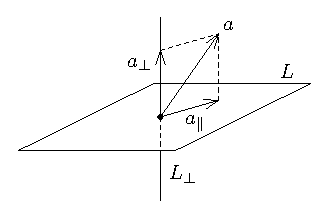
\includegraphics[width=0.35\textwidth]{6_1.eps}
	\label{6_1}
	\caption{Ортогональная проекция.}
	\label{fig:Ортогональная проекция}
\end{figure}

\end{document}